\subsubsection{Risultati sperimentali}
% TODO: describe figs
\autoref{fig:obj2_boxplot_population} mostra la distribuzione della Popolazione media al variare del rate medio di arrivi esterni per ogni nodo del sistema e globale. È possibile notare come l'andamento assuma una forma esponenziale.

\autoref{fig:obj2_lineplots_rtime} mostra la distribuzione del Tempo di Risposta medio al variare del rate medio di arrivi esterni per ogni nodo del sistema e globale. È possibile notare come l'andamento assuma una forma esponenziale, con una maggiore variabilità corrispondente ai rate di arrivo più alti.

\autoref{fig:obj2_boxplot_throughput} mostra la distribuzione del Throughput medio al variare del rate medio di arrivi esterni per ogni nodo del sistema e globale. Il throughput sembra crescere linearmente all'aumentare del rate, segno che il sistema rimane stabile fino a $1.2 req/s$. Il throughput del sistema sembra avere una leggera flessione verso il basso verso i rate più alti, segno che il sistema, pur rimanendo stabile, si avvicina al punto di saturazione.

\autoref{fig:obj2_boxplot_utilization} mostra la distribuzione dell'Utilizzazione media al variare del rate medio di arrivi esterni per ogni nodo del sistema e globale. L'Utilizzazione del sistema sembra crescere linearmente all'aumentare del rate, fino a colpire il tetto massimo di $1$ nei rate più alti, il che spiegherebbe l'alta variabilità del tempo di risposta in prossimità di tali rates.

\begin{figure*}
    \centering
    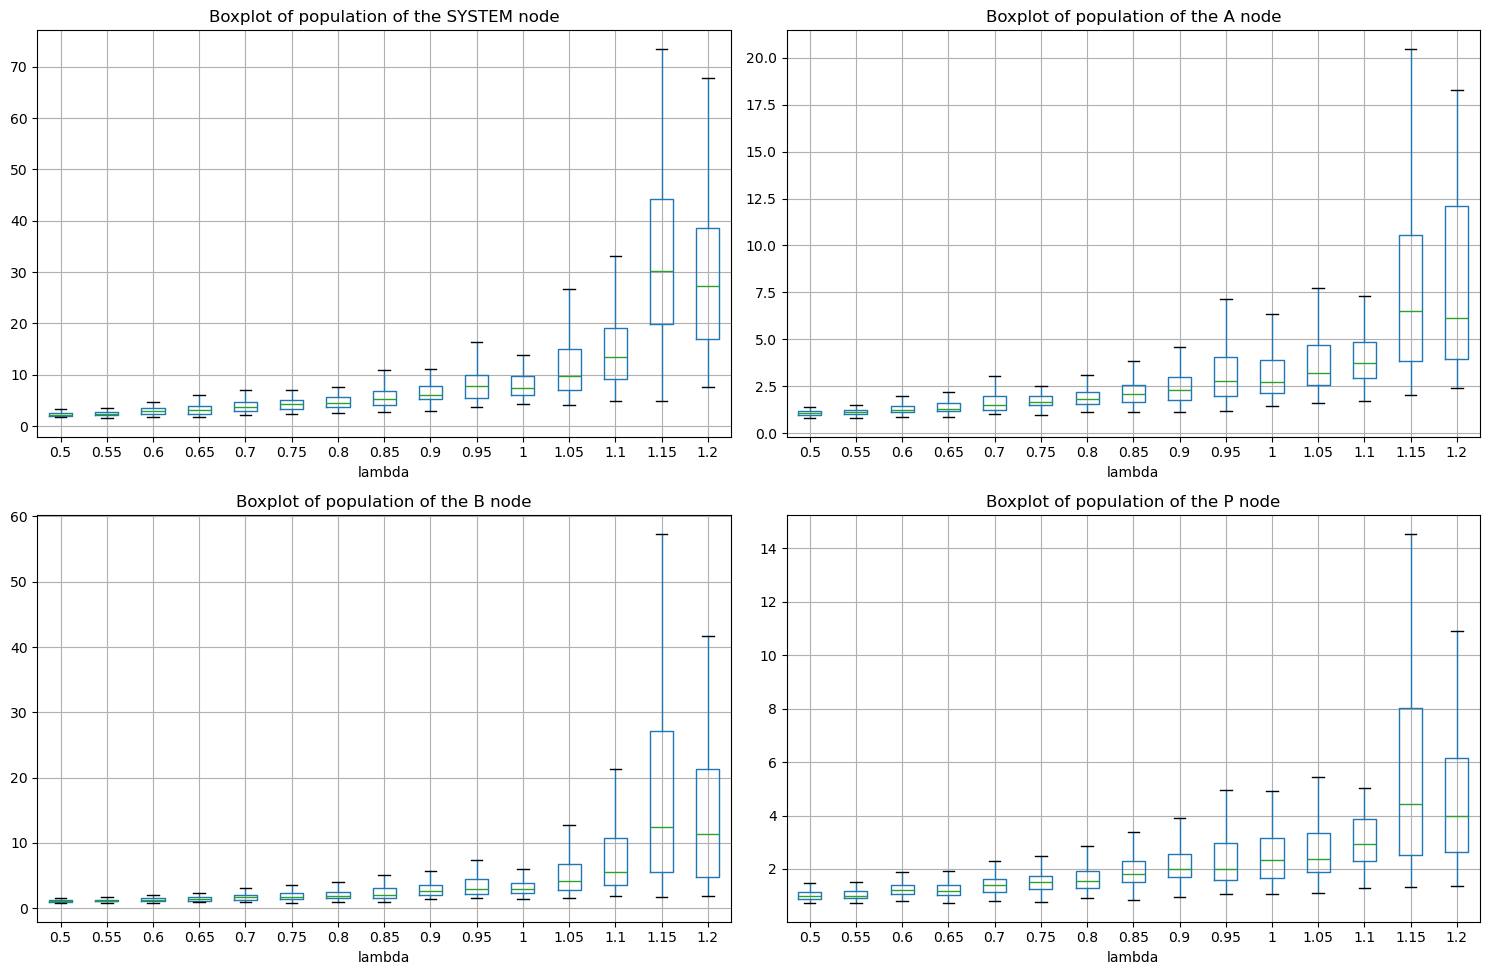
\includegraphics[width=1\linewidth]{figs//results/obj2/simulation/obj2_boxplot_population.png}
    \caption{Distribuzione della popolazione media dei risultati sperimentali dell'obbiettivo 2.}
    \label{fig:obj2_boxplot_population}
\end{figure*}

\begin{figure*}
    \centering
    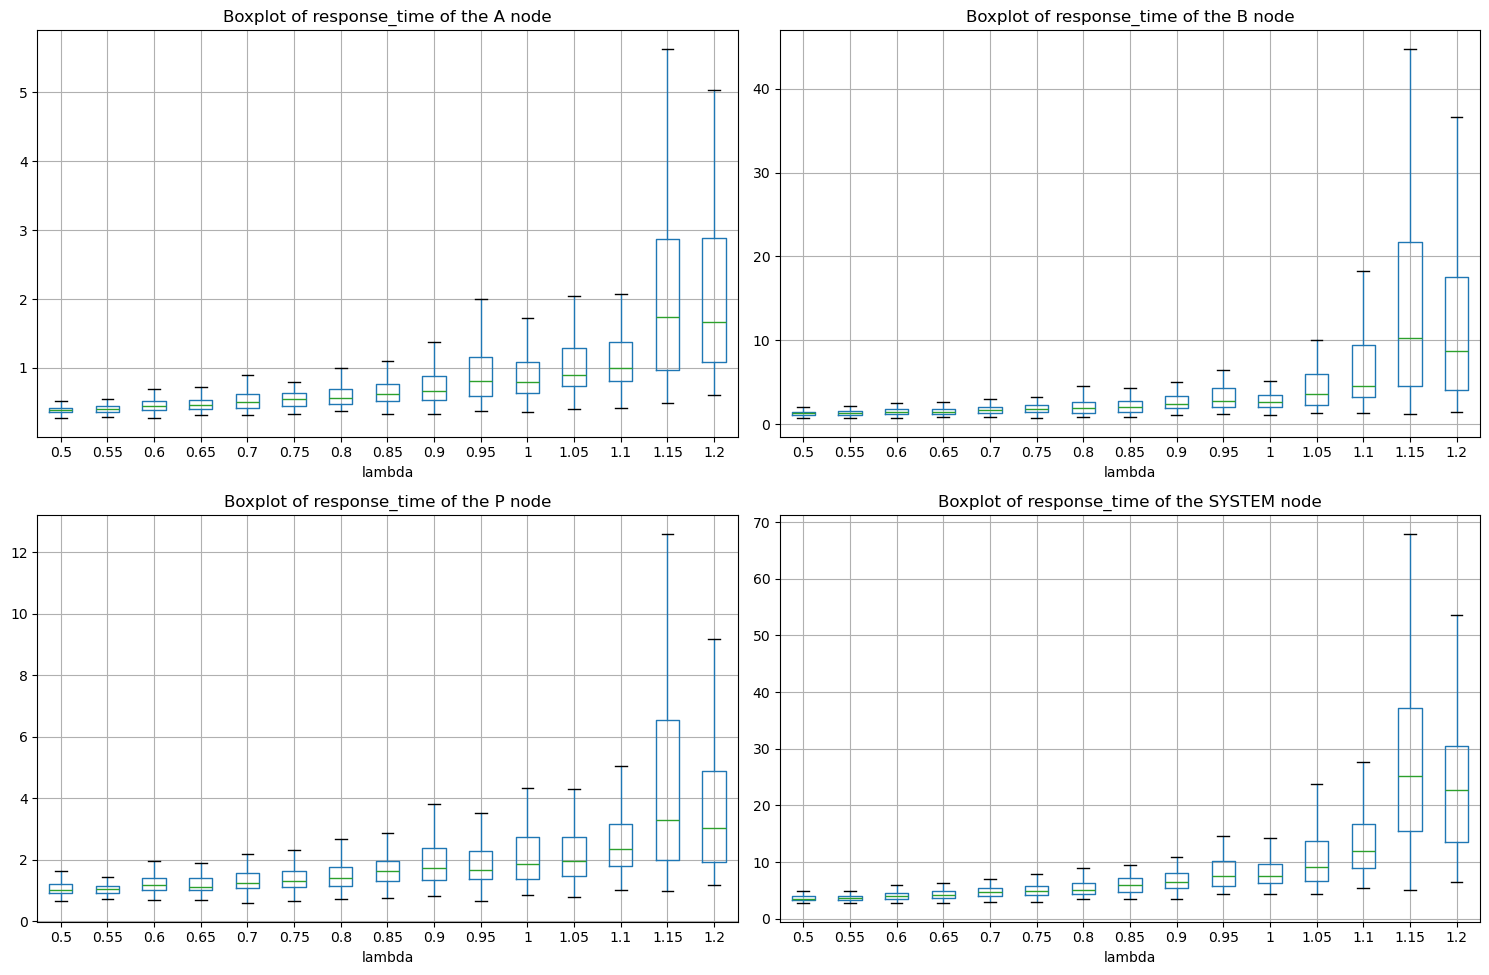
\includegraphics[width=1\linewidth]{figs//results/obj2/simulation/obj2_boxplot_rtime.png}
    \caption{Distribuzione del Tempo di Risposta medio dei risultati sperimentali dell'obbiettivo 2.}
    \label{fig:obj2_boxplot_rtime}
\end{figure*}

\begin{figure*}
    \centering
    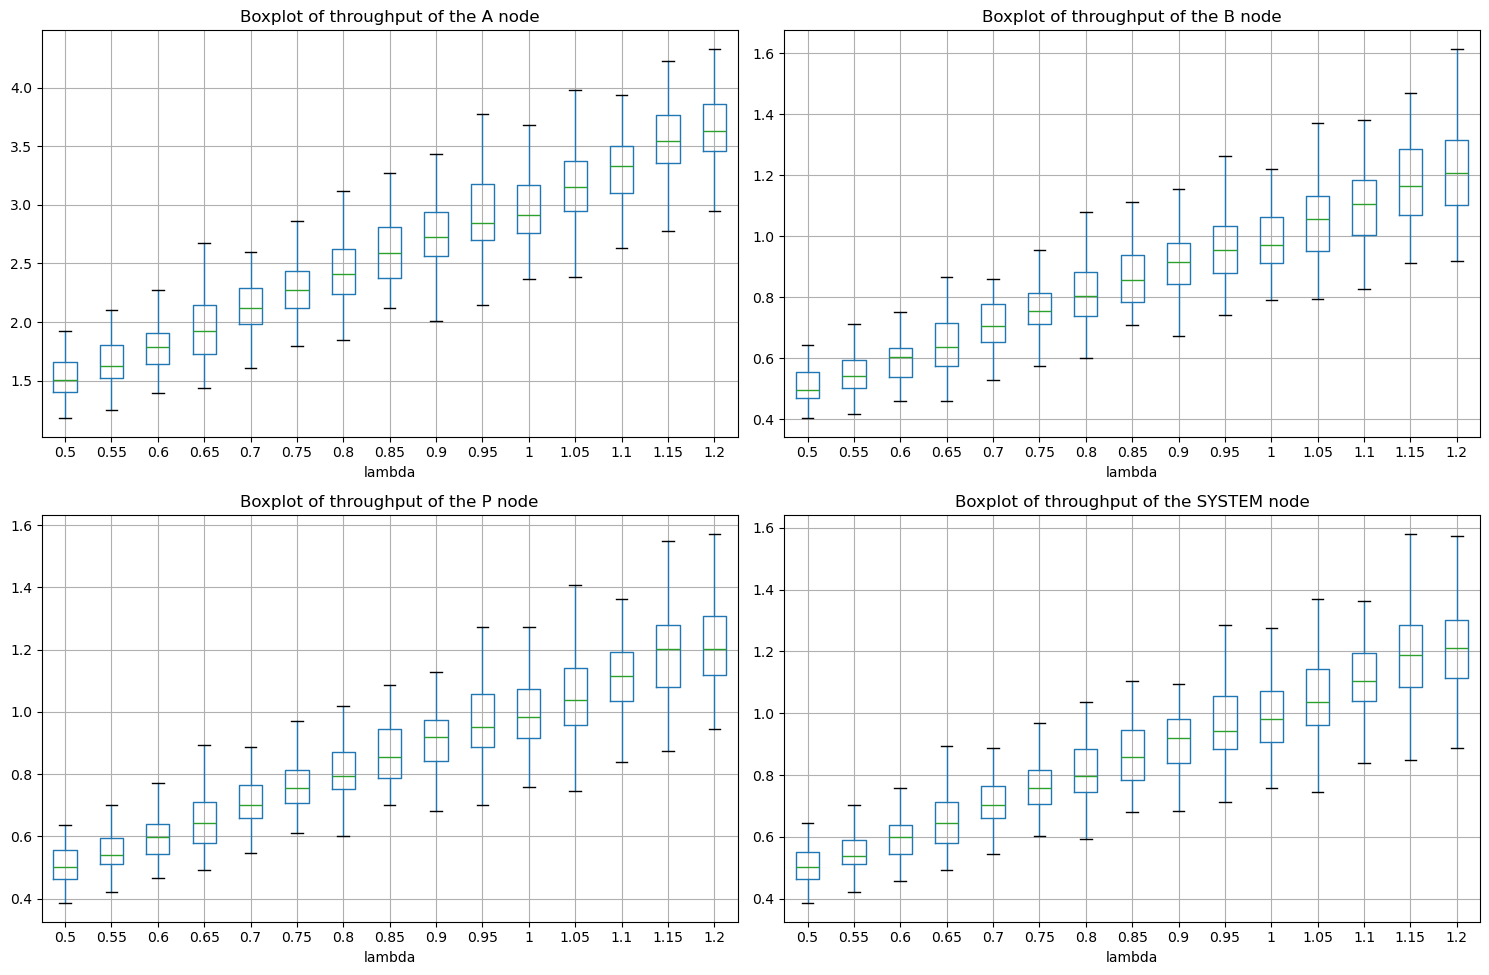
\includegraphics[width=1\linewidth]{figs/results/obj2/simulation/obj2_boxplot_throughput.png}
    \caption{Distribuzione del Throughput medio dei risultati sperimentali dell'obbiettivo 2.}
    \label{fig:obj2_boxplot_throughput}
\end{figure*}

\begin{figure*}
    \centering
    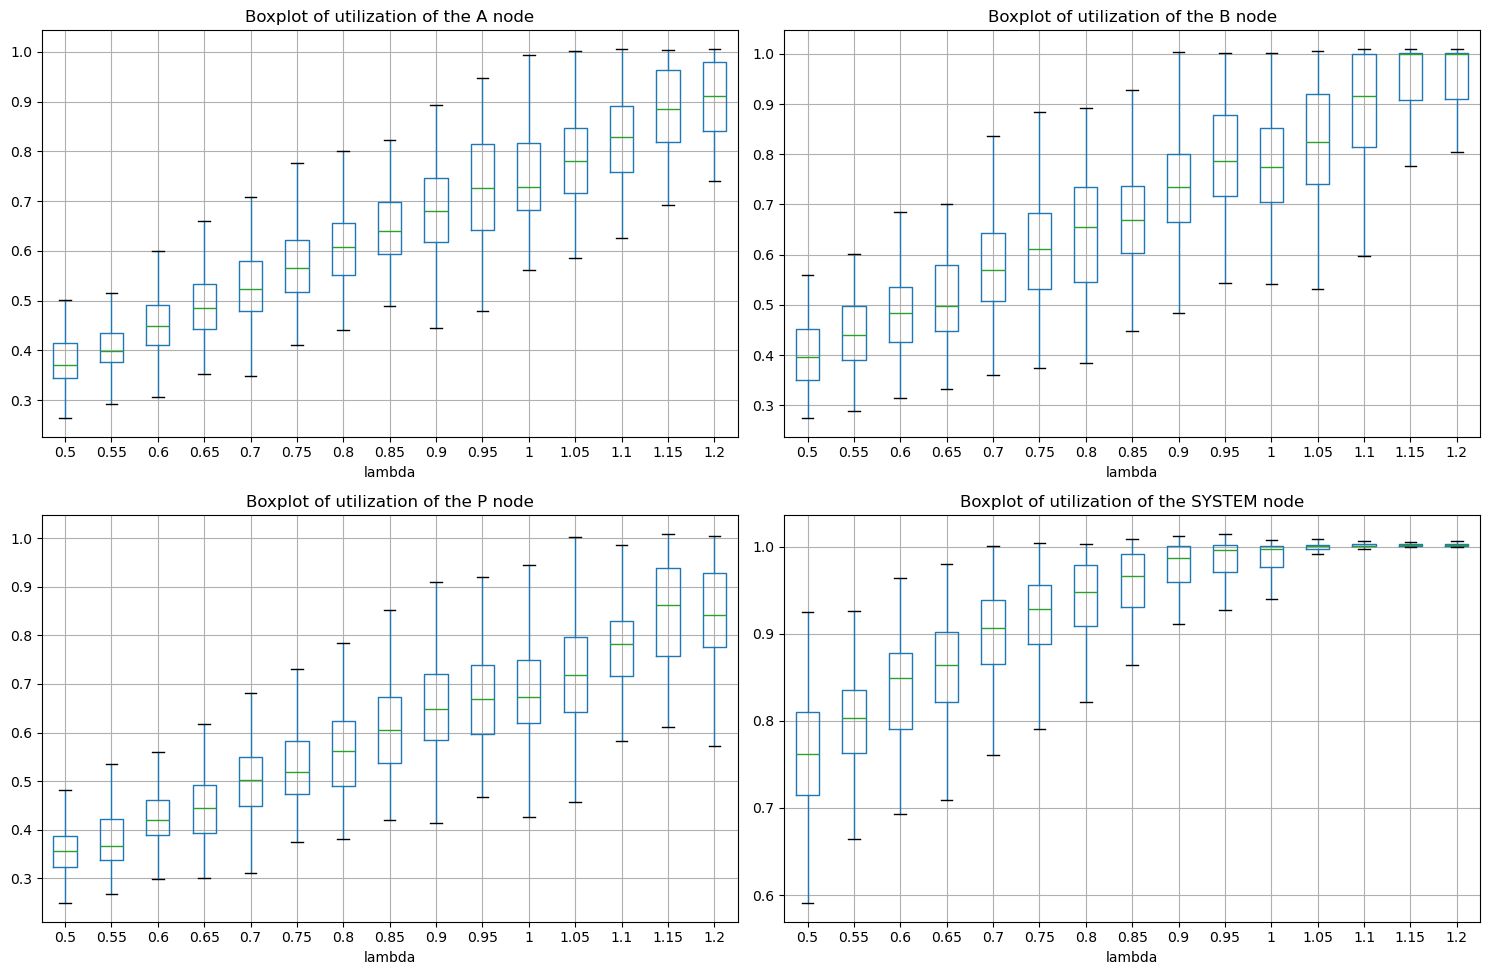
\includegraphics[width=1\linewidth]{figs//results/obj2/simulation/obj2_boxplot_utilization.png}
    \caption{Distribuzione dell'Utilizzatione media dei risultati sperimentali dell'obbiettivo 2.}
    \label{fig:obj2_boxplot_utilization}
\end{figure*}

\subsubsection{Verifica con il modello analitico}
\label{sec:results_obj2_verication}
\autoref{fig:obj2_lineplots_population},\autoref{fig:obj2_lineplots_rtime}, \autoref{fig:obj2_lineplots_throughput}, e  mostrano l'allineamento dei valori sperimentali di Popolazione, Tempo di Risposta e Throughput medi con quelli teorici forniti dal modello analitico. È opportuno notare che il modello analitico è stato definito modellando il Server A senza tener conto che job di classe diversa hanno tempi medi di servizio diversi, per cui è possibile notare delle discrepanze sopratutto per le metriche del Server A. Infatti, l'effetto finale è che il modello analitico risulta essere "ottimista" rispetto ai risultati di simulazione.

\autoref{fig:obj2_lineplots_utilization} mostra l'allineamento dei valori sperimentali \\dell'Utilizzazione media con quelli teorici forniti dal modello analitico dei server A, B, P. In \autoref{fig:obj2_lineplots_utilization_A} si vede ancora una volta come il modello analitico sia ottimista rispetto ai valori sperimentali.

\begin{figure*}
    \centering
    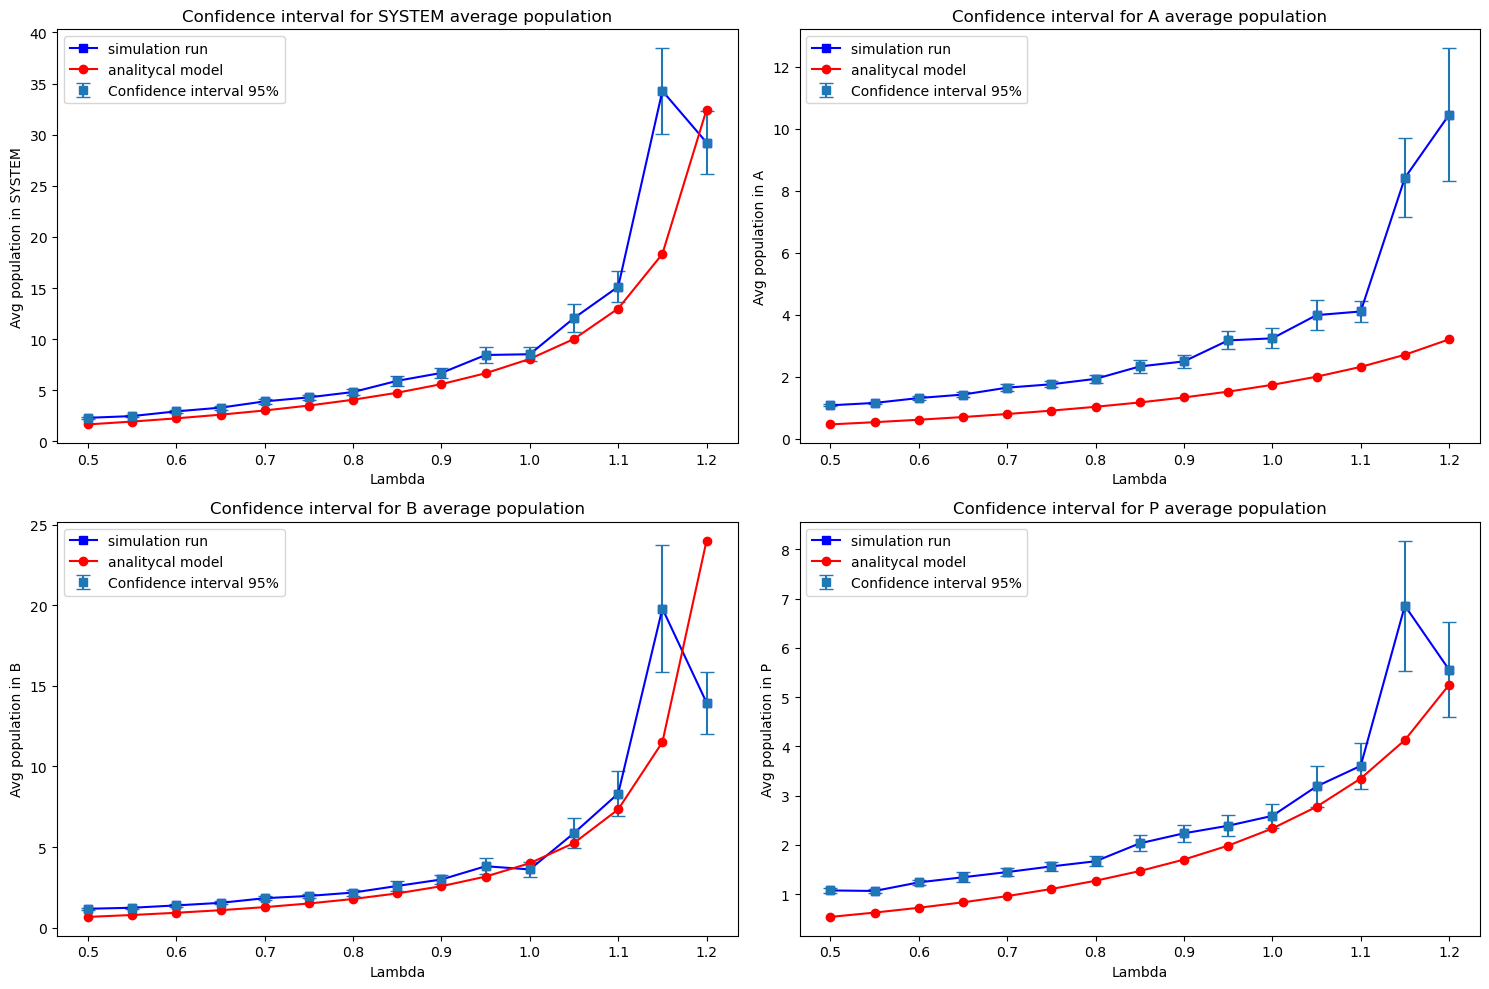
\includegraphics[width=1\linewidth]{figs//results//obj2//verification/obj2_lineplots_population.png}
    \caption{Confronto tra valori medi della simulazione e del modello analitico della Popolazione per l'Obiettivo 2.}
    \label{fig:obj2_lineplots_population}
\end{figure*}

\begin{figure*}
    \centering
    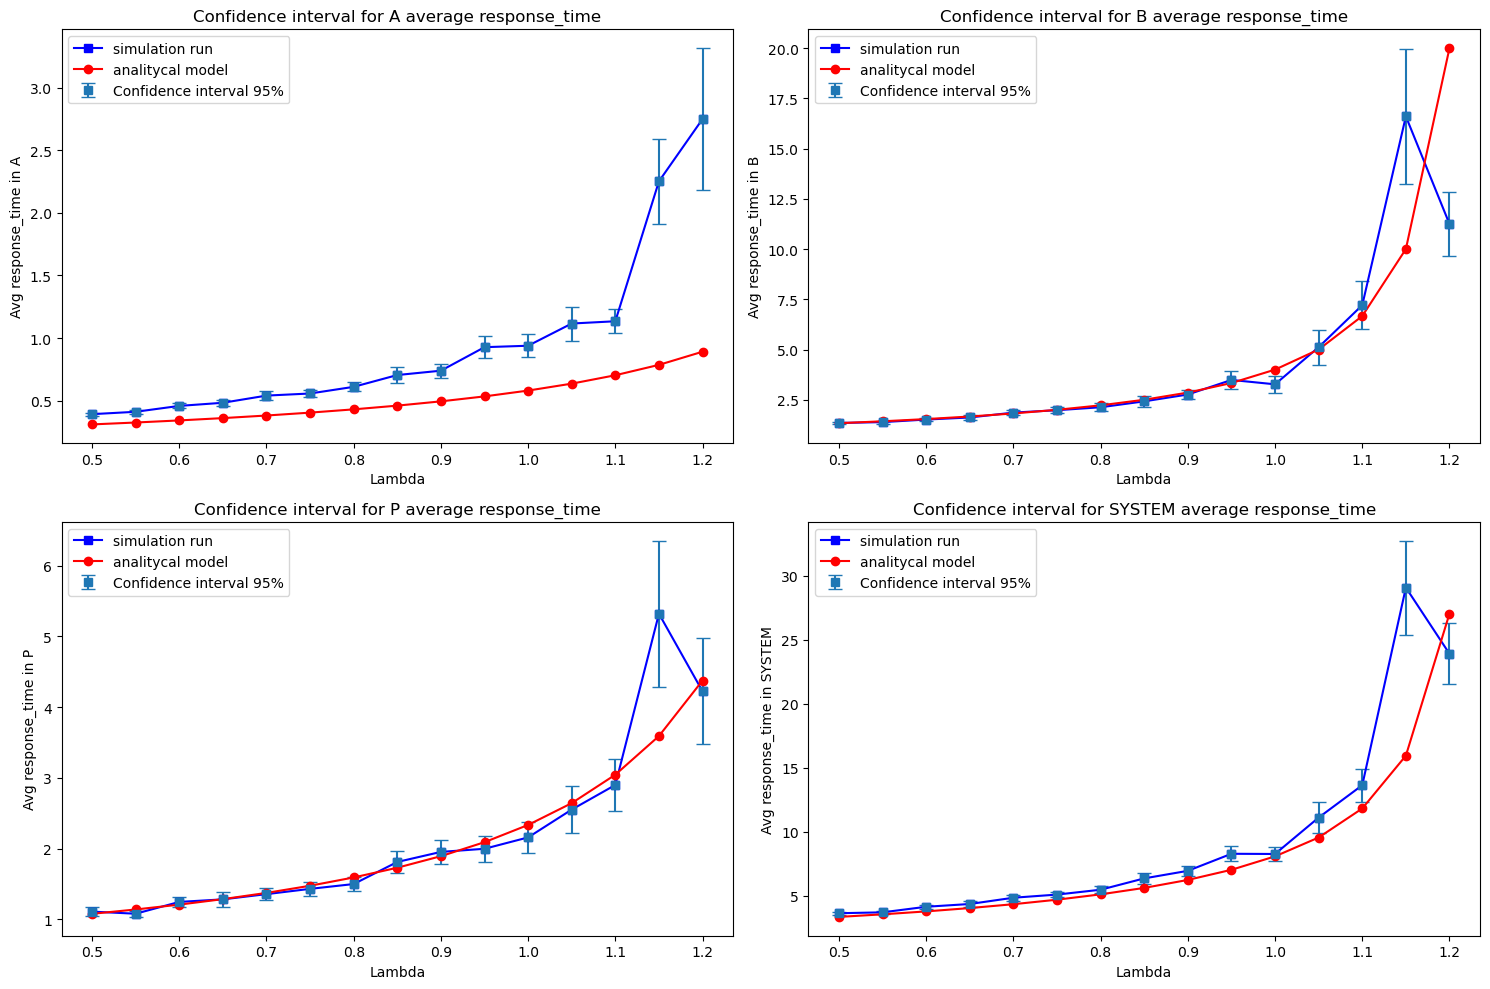
\includegraphics[width=1\linewidth]{figs//results//obj2//verification/obj2_lineplots_rtime.png}
    \caption{Confronto tra valori medi della simulazione e del modello analitico dell Tempo di Risposta per l'Obiettivo 2.}
    \label{fig:obj2_lineplots_rtime}
\end{figure*}

\begin{figure*}
    \centering
    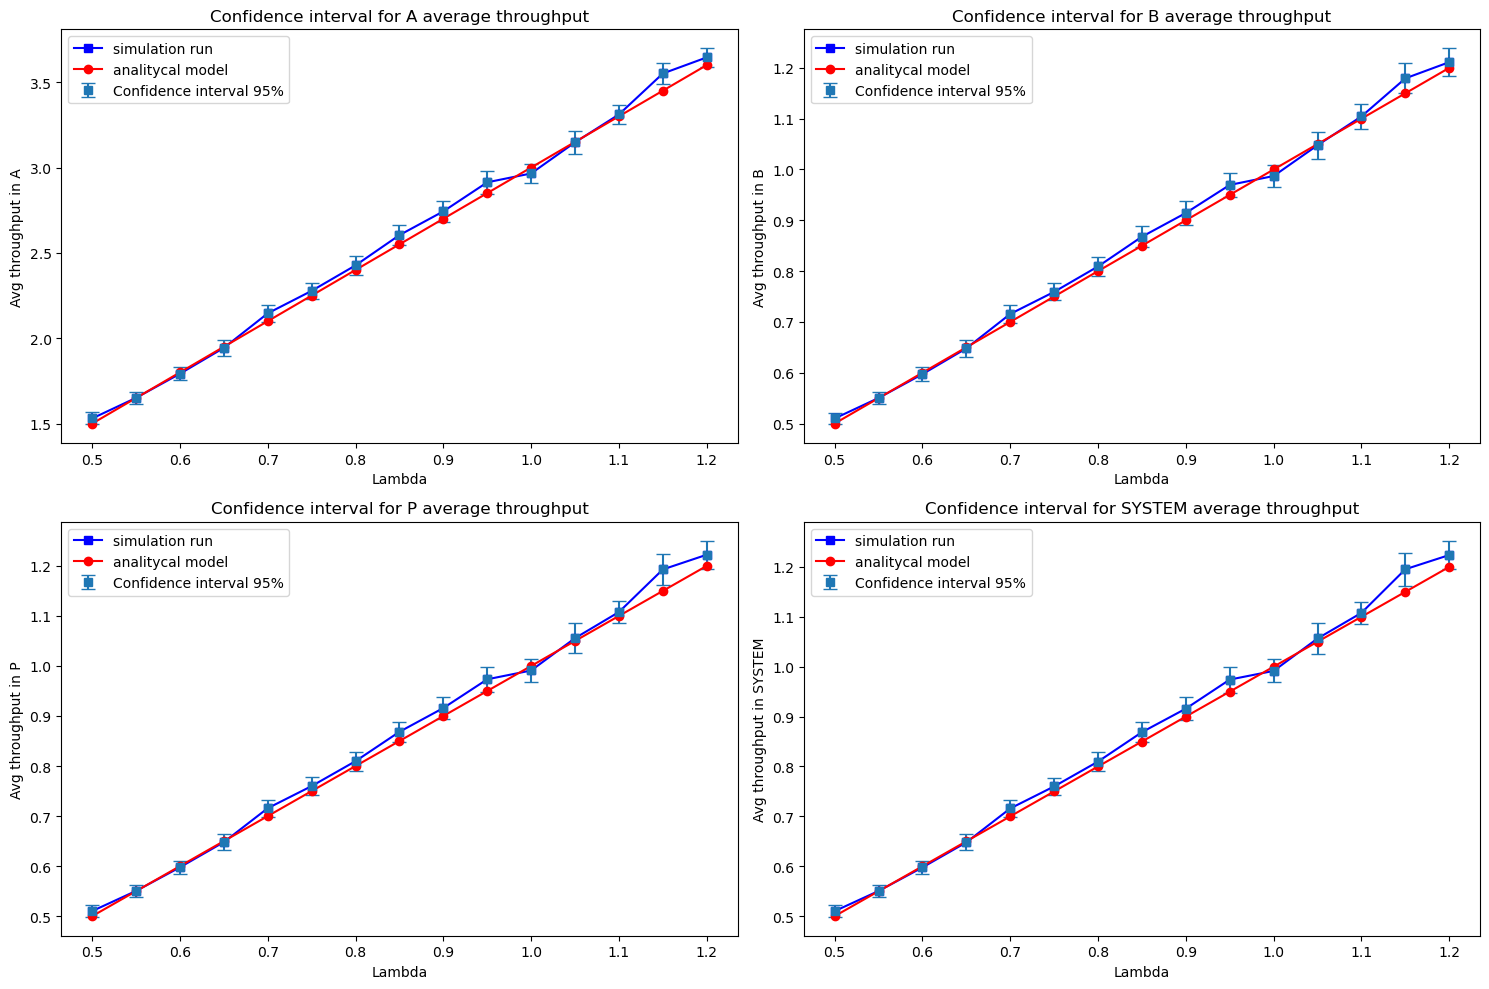
\includegraphics[width=1\linewidth]{figs/results/obj2/verification/obj2_lineplots_throughput.png}
    \caption{Confronto tra valori medi della simulazione e del modello analitico del Throughput per l'Obiettivo 2.}
    \label{fig:obj2_lineplots_throughput}
\end{figure*}

% line plots utilizzazione
\begin{figure*}
    \centering
    \begin{subfigure}{0.49\linewidth}
        \centering
        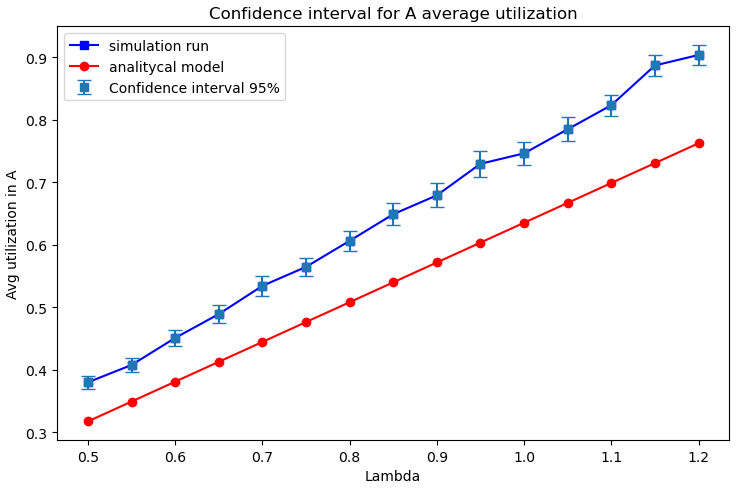
\includegraphics[width=1\linewidth]{figs//results//obj2//verification/obj2_lineplots_utilization_A.png}
        \caption{Server A.}
        \label{fig:obj2_lineplots_utilization_A}
    \end{subfigure} 
    \begin{subfigure}{0.49\linewidth}
        \centering
        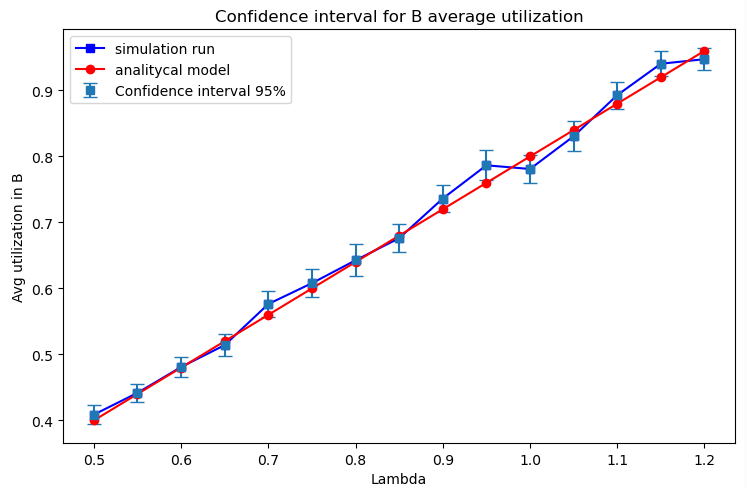
\includegraphics[width=1\linewidth]{figs//results//obj2//verification/obj2_lineplots_utilization_B.png}
        \caption{Server B.}
        \label{fig:obj2_lineplots_utilization_B}
    \end{subfigure}
    \begin{subfigure}{0.5\linewidth}
        \centering
        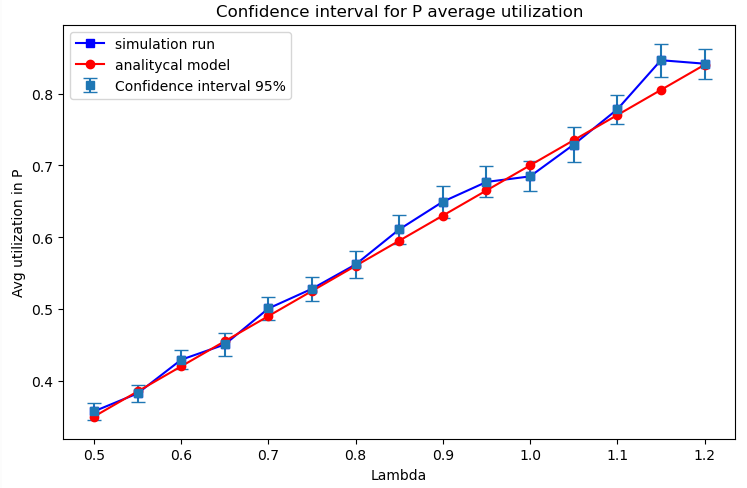
\includegraphics[width=1\linewidth]{figs//results//obj2//verification/obj2_lineplots_utilization_P.png}
        \caption{Server P.}
        \label{fig:obj2_lineplots_utilization_P}
    \end{subfigure}
    \caption{Confronto tra valori medi della simulazione e del modello analitico dell'Utilizzazione per l'Obiettivo 2.}
    \label{fig:obj2_lineplots_utilization}
\end{figure*}

% \textbf{Modello analitico utilizzazione}\\
\begin{table}[!htbp]
    \centering
    \begin{tabular}{cccc}
        $\gamma$ & $\rho_{A}$ & $\rho_{B}$ & $\rho_{P}$ \\         
        0.5 & 0.317 & 0.4 & 0.35 \\
        1.2 & 0.762 & 0.96 & 0.84 \\
    \end{tabular}
    \label{tab:rho_values}
\end{table}

\textbf{Modello analitico indici locali}\\

\begin{table}[!htbp]
    \centering
    \begin{tabular}{cccc}
        $\gamma$ & $E[T]_{A}$ & $E[T]_{B}$ & $E[T]_{P}$ \\         
        0.5 & 0.310 & 1.333 & 1.076 \\
        1.2 & 0.891 & 20 & 4.375 \\
    \end{tabular}
    \label{tab:et_values}
\end{table}
\begin{table}[!htbp]
    \centering
    \begin{tabular}{cccc}
        $\gamma$ & $E[N]_{A}$ & $E[N]_{B}$ & $E[N]_{P}$ \\         
        0.5 & 0.465 & 0.666 & 0.538 \\
        1.2 & 3.207 & 24 & 5.25 \\
    \end{tabular}
    \label{tab:en_values}
\end{table}
\begin{table}[!htbp]
    \centering
    \begin{tabular}{cccc}
        $\gamma$ & $X_{A}$ & $X_{B}$ & $X_{P}$ \\         
        0.5 & 1.5 & 0.5 & 0.5 \\
        1.2 & 3.6 & 1.2 & 1.2 \\
    \end{tabular}
    \label{tab:x_values}
\end{table}

\textbf{Modello analitico indici globali}
\begin{table}[!htbp]
    \centering
    \begin{tabular}{cccc}
        $\gamma$ & $E[T]_{S}$ & $E[N]_{S}$ & $X_{S}$ \\         
        0.5 & 3.341 & 1.670 & 0.5 \\
        1.2 & 27.048 & 32.457 & 1.2 \\
    \end{tabular}
    \label{tab:et_en_x_values_last}
\end{table}


\subsubsection{Validazione con il caso di studio}
\label{sec:results_obj2_validation}
\autoref{fig:Single_VS_Two_FA_Perfomance_Comparison} riporta i valori medi del Tempo di Risposta e della Popolazione ottenuti tramite il nostro simulatore confrontati con i valori riportati da \citet{DBLP:books/sp/Serazzi24}. È possibile notare come in entrambi i risultati le metriche di performance siano più alte con la two-factor authentication rispetto alla single-factor. Inoltre, gli andamenti sembrano essere tutti esponenziali. I risultati sembrano essere in linea con quanto riportato nel caso di studio.

\begin{figure*}
    \centering
    \begin{subfigure}[b]{0.49\linewidth}
        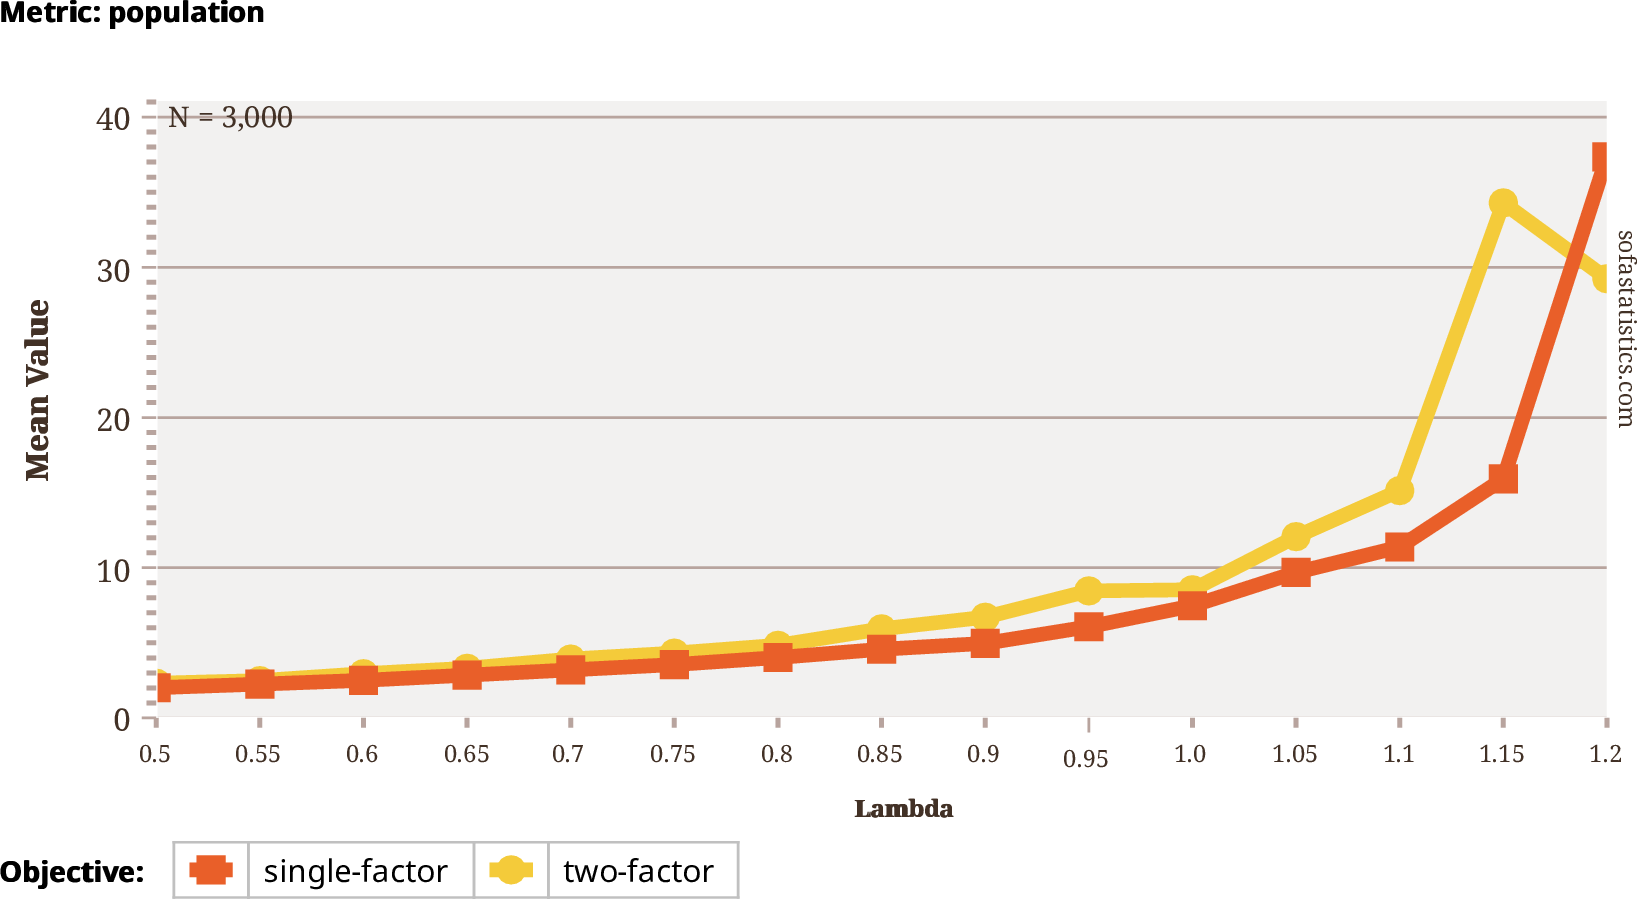
\includegraphics[width=1\linewidth]{figs/results/obj2/validation/single_VS_Two_FA_Perfomance_Comparison_population.png}
        \caption{Popolazione}
        \label{fig:Single_VS_Two_FA_Perfomance_Comparison_population}
    \end{subfigure}
    \hfill
    \begin{subfigure}[b]{0.49\linewidth}
        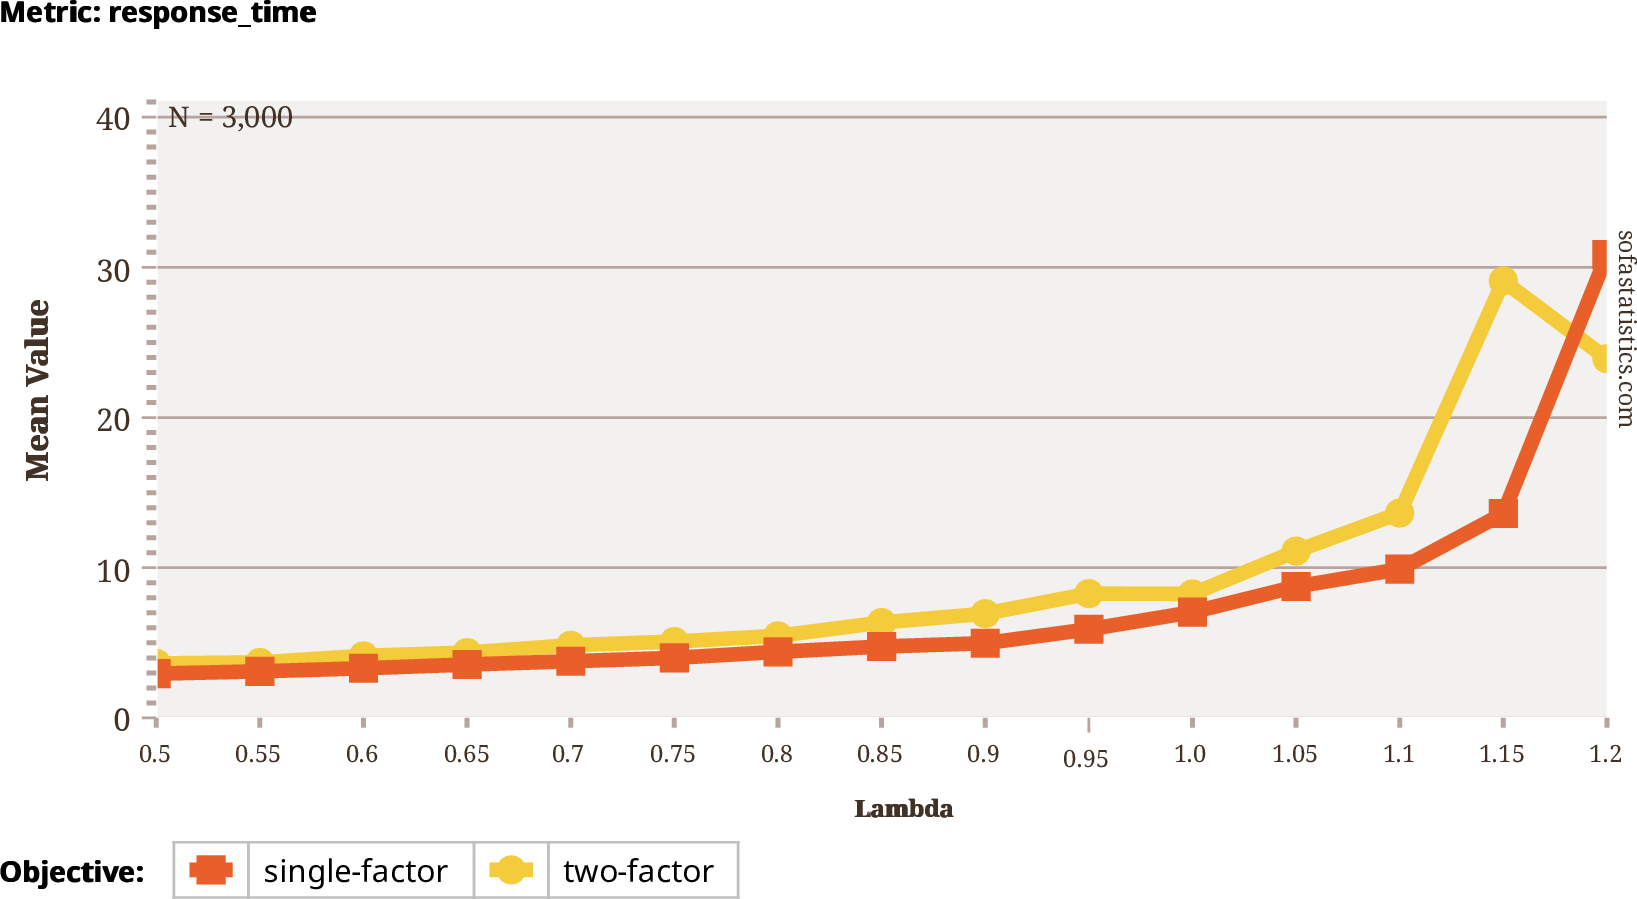
\includegraphics[width=1\linewidth]{figs/results/obj2/validation/single_VS_Two_FA_Perfomance_Comparison_rtime.png}
        \caption{Tempo di Risposta}
        \label{fig:Single_VS_Two_FA_Perfomance_Comparison_rtime}
    \end{subfigure}
    \hfill
    \begin{subfigure}{1\linewidth}
        \centering
        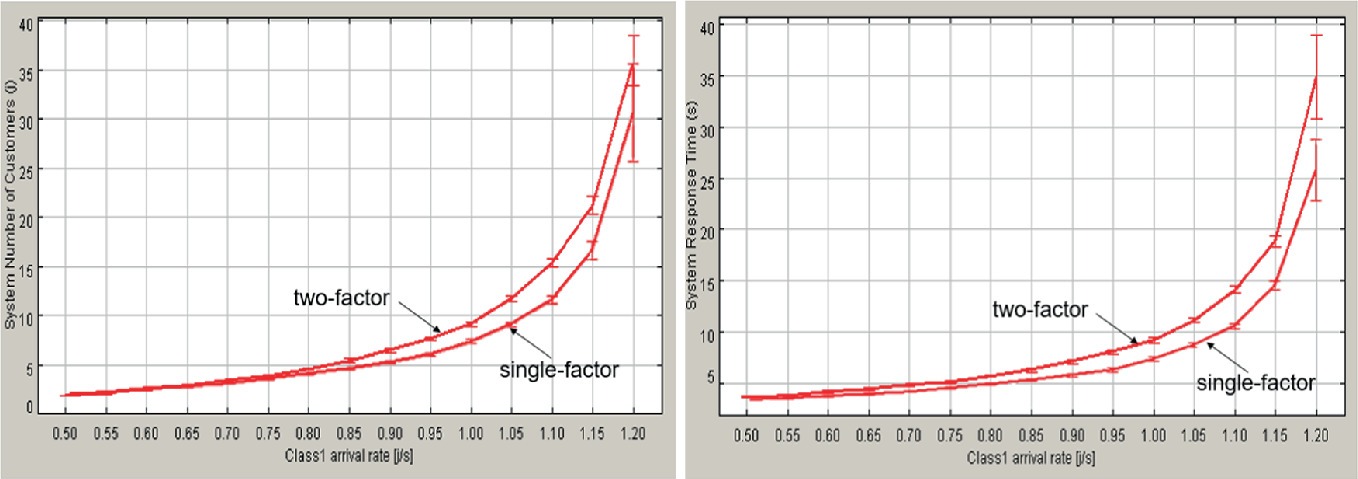
\includegraphics[width=1\linewidth]{figs//results//obj2//validation/casestudy_system_rtime_population.png}
        \caption{Popolazione media (sinistra) e Tempo di Risposta medio (destra) \citep{DBLP:books/sp/Serazzi24}.}
        \label{fig:casestudy_system_rtime_population}
    \end{subfigure}
    \caption{Popolazione e Tempo di Risposta medi del sistema in funzione del rate di arrivi esterni nel caso con e senza 2FA.}
    \label{fig:Single_VS_Two_FA_Perfomance_Comparison}
\end{figure*}